\subsection{Example of real-life situations}

As we said before, the MEWC has many real-world applications in various fields
such as social networks, chemistry, bioinformatics. Now, we will give an concrete
example of a real-life situation that can be modelled as a MEWC problem. \newline

\textbf{The team formation process} for a project, or for the search for a particular
social group, is a situation that can be viewed as a MEWC problem. Let's imagine that
the Student Office of ISEN Nantes is looking to reinforce the video games club of its
school. Indeed, the latter has no succession for the following year and is thus led to
die if no member presents himself. The future members of the office will have to be
in contact with each other during a whole year and it is thus important to find people
with common interests so that no tension is formed during their studies. The office has
access to the Steam profiles of the students within ISEN (Steam is a video game digital
distribution service that gives information about the games played by each one) as well
as a record made by the gaming club of the different games played by their members. The
fact of playing games in common could bring some people closer, and this makes it a good
criterion to create a group that could take over the club because it would share common
interests. \newline

To model this problem, we can represent each student as a vertex and each the games
played in common as an edge. The weight of each edge will be the number of games played
in common. The goal of the office is to find a group of students that will take over the
club. To do this, we will use the MEWC algorithm to find a group of students that
has the highest affinity. \newline

In the following example, we will restrict ourselves to 9 students of the CIR3 class
of ISEN Nantes since it would be too complicated to represent every student of the
school. We will also assume that the students have played the game listed in the table
below. \newline

\rowcolors{2}{gray!10}{gray!30}
\begin{tabular}{|p{0.3\textwidth}|p{0.65\textwidth}|}
    \hline
    \textbf{Students} & \textbf{Game played}                         \\
    \hline
    Youn              & Minecraft, Civilisations, Lost ARK, Among US \\
    Martin            & Minecraft                                    \\
    Valentin          & Genshin, Minecraft, Civilisations            \\
    Bastien           & Genshin, Minecraft, Lost ARK, Among US       \\
    Guillaume         & CSGO, Genshin, Overwatch, Stardew Valley     \\
    Dorian            & CSGO, Paladins, Overwatch                    \\
    Antoine           & League of Legends, Stardew Valley            \\
    Thomas            & League of Legends, The Last of US            \\
    Alexandre         & League of Legends, Dofus                     \\
    \hline
\end{tabular}
\rowcolors{1}{}{}
\vspace{1\baselineskip} \\
Which would give us this graph :

\begin{figure}[H]
    \centering
    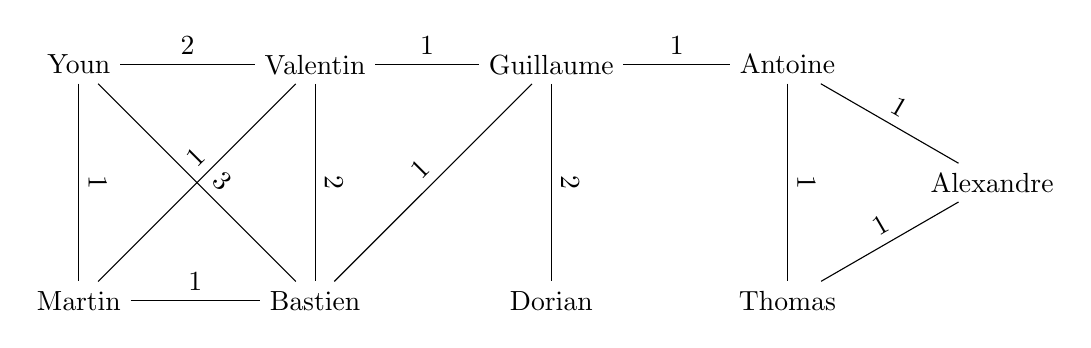
\begin{tikzpicture}[node distance=3cm]
        \node (youn) {Youn};
        \node (valentin) [right of=youn] {Valentin};
        \node (guillaume) [right of=valentin] {Guillaume};
        \node (antoine) [right of=guillaume] {Antoine};
        \node (martin) [below of=youn] {Martin};
        \node (bastien) [right of=martin] {Bastien};
        \node (dorian) [right of=bastien] {Dorian};
        \node (thomas) [right of=dorian] {Thomas};
        \node (alexandre) at ([shift=(-30:3)] antoine) {Alexandre};

        \draw (youn)
        edge node[above, sloped] {$2$} (valentin)
        edge node[above, sloped] {$1$} (martin)
        edge node[above right, sloped] {$3$} (bastien);
        \draw (valentin)
        edge node[above right, sloped] {$1$} (martin)
        edge node[above, sloped] {$2$} (bastien)
        edge node[above, sloped] {$1$} (guillaume);
        \draw (martin)
        edge node[above, sloped] {$1$} (bastien);
        \draw (guillaume)
        edge node[above, sloped] {$1$} (bastien)
        edge node[above, sloped] {$2$} (dorian)
        edge node[above, sloped] {$1$} (antoine);
        \draw (antoine)
        edge node[above, sloped] {$1$} (thomas)
        edge node[above, sloped] {$1$} (alexandre);
        \draw (thomas)
        edge node[above,sloped] {$1$} (alexandre);
    \end{tikzpicture}
    \caption{Graph representing the games played between the students}
\end{figure}

The goal of the Maximum Edge Weight Clique problem in this context would be to
find a complete subset of individuals such that the sum of the weights of the
edges between the individuals is maximized. In this example, the maximum weight
clique would be the clique consisting of nodes Youn, Valentin, Martin, Bastien
with a total weight of $2+1+1+1+3+2=10$.